\documentclass[10pt,a4paper]{article}
\usepackage[utf8]{inputenc}\usepackage[T1]{fontenc}\usepackage[brazil]{babel}
\usepackage{geometry,graphicx,amsmath,booktabs,microtype}
\geometry{margin=1.65cm}\setlength{\parindent}{0pt}\setlength{\parskip}{3pt}
\title{\vspace{-1em}\textbf{Diagnóstico probabilístico de falhas industriais}\\\large Projeto 1 — Rede Bayesiana}
\author{Portfólio de Inteligência Artificial 1}\date{}
\begin{document}\maketitle\vspace{-1em}
\textbf{Resumo.} Este projeto modela uma máquina industrial por uma Rede Bayesiana binária e realiza inferência exata por enumeração. A contribuição é uma estrutura causal não trivial que separa causas latentes (desgaste, sobrecarga e lubrificação) dos sintomas e dos modos de falha.
\section{Problema e modelagem}
Sensores industriais são ruidosos e uma mesma evidência pode ter causas concorrentes. O objetivo é estimar $P(\text{falha}\mid\text{evidências})$ em quatro cenários: normal, temperatura/vibração altas, indícios elétricos e múltiplas evidências. O DAG contém oito variáveis: desgaste, lubrificação insuficiente, sobrecarga, temperatura alta, vibração alta, pressão inadequada, falha mecânica e falha elétrica. A direção foi escolhida para representar causas operacionais a montante e sintomas observáveis a jusante.
\begin{figure}[h]\centering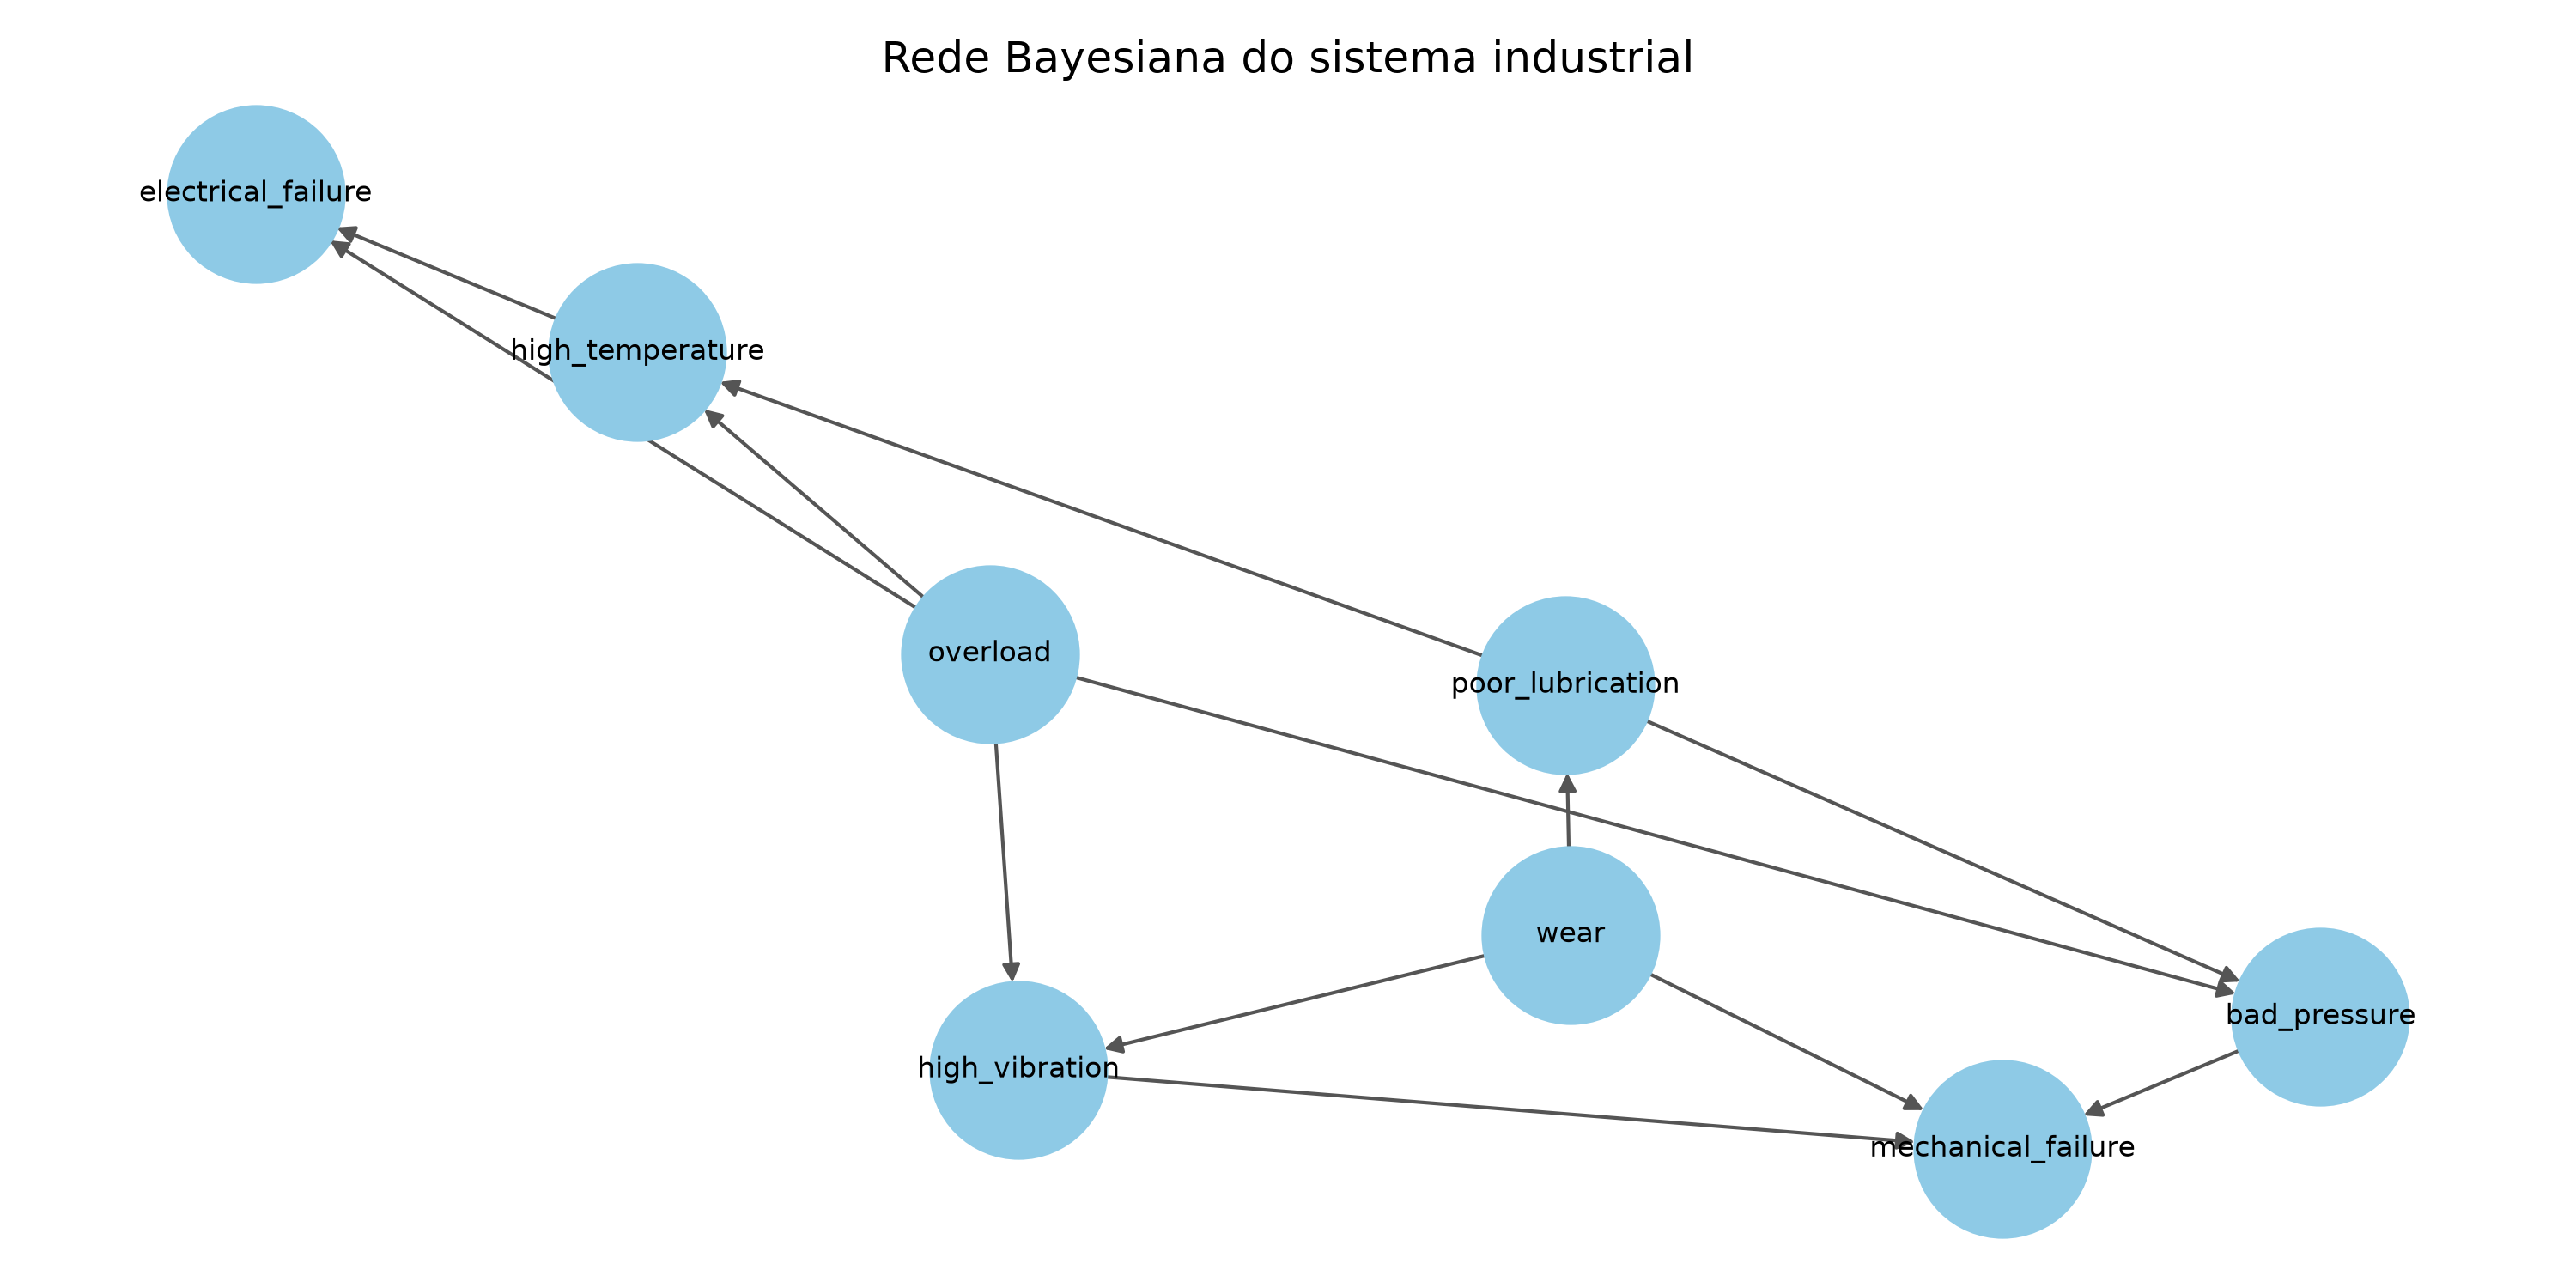
\includegraphics[width=.72\linewidth]{results/bayesian_network.png}\caption{DAG implementado.}\end{figure}
\section{Fundamentação e algoritmo}
Para uma atribuição completa $\mathbf{x}$, a fatoração usada é
\[
 P(\mathbf{x})=\prod_i P(x_i\mid \mathrm{pais}(X_i)).
\]
Para uma consulta $Q$ e evidência $\mathbf{e}$, o programa enumera as variáveis ocultas:
\[
 P(Q\mid\mathbf{e})=\frac{\sum_{\mathbf{y}}P(Q,\mathbf{e},\mathbf{y})}
 {\sum_{q,\mathbf{y}}P(q,\mathbf{e},\mathbf{y})}.
\]
As CPTs foram definidas manualmente com probabilidades maiores sob desgaste e sobrecarga. O método verifica ciclos, nós desconhecidos, normalização implícita de cada Bernoulli e evidência impossível. Assim, a implementação expõe o mecanismo matemático, sem delegar inferência a biblioteca.
\section{Experimentos e resultados}
A semente não é necessária na inferência, pois a rede é determinística. A tabela registra a saída real em \texttt{results/metrics.json}.
\begin{center}\small
\begin{tabular}{lrrrr}\toprule
Cenário & Mecânica & Elétrica & Desgaste & Sobrecarga\\\midrule
Normal & 0,147 & 0,068 & 0,180 & 0,150\\
Temperatura+vibração & 0,628 & 0,445 & 0,552 & 0,715\\
Indícios elétricos & 0,036 & 0,308 & 0,159 & 0,346\\
Múltiplas evidências & 0,824 & 0,472 & 0,625 & 0,789\\\bottomrule
\end{tabular}\end{center}
\begin{figure}[h]\centering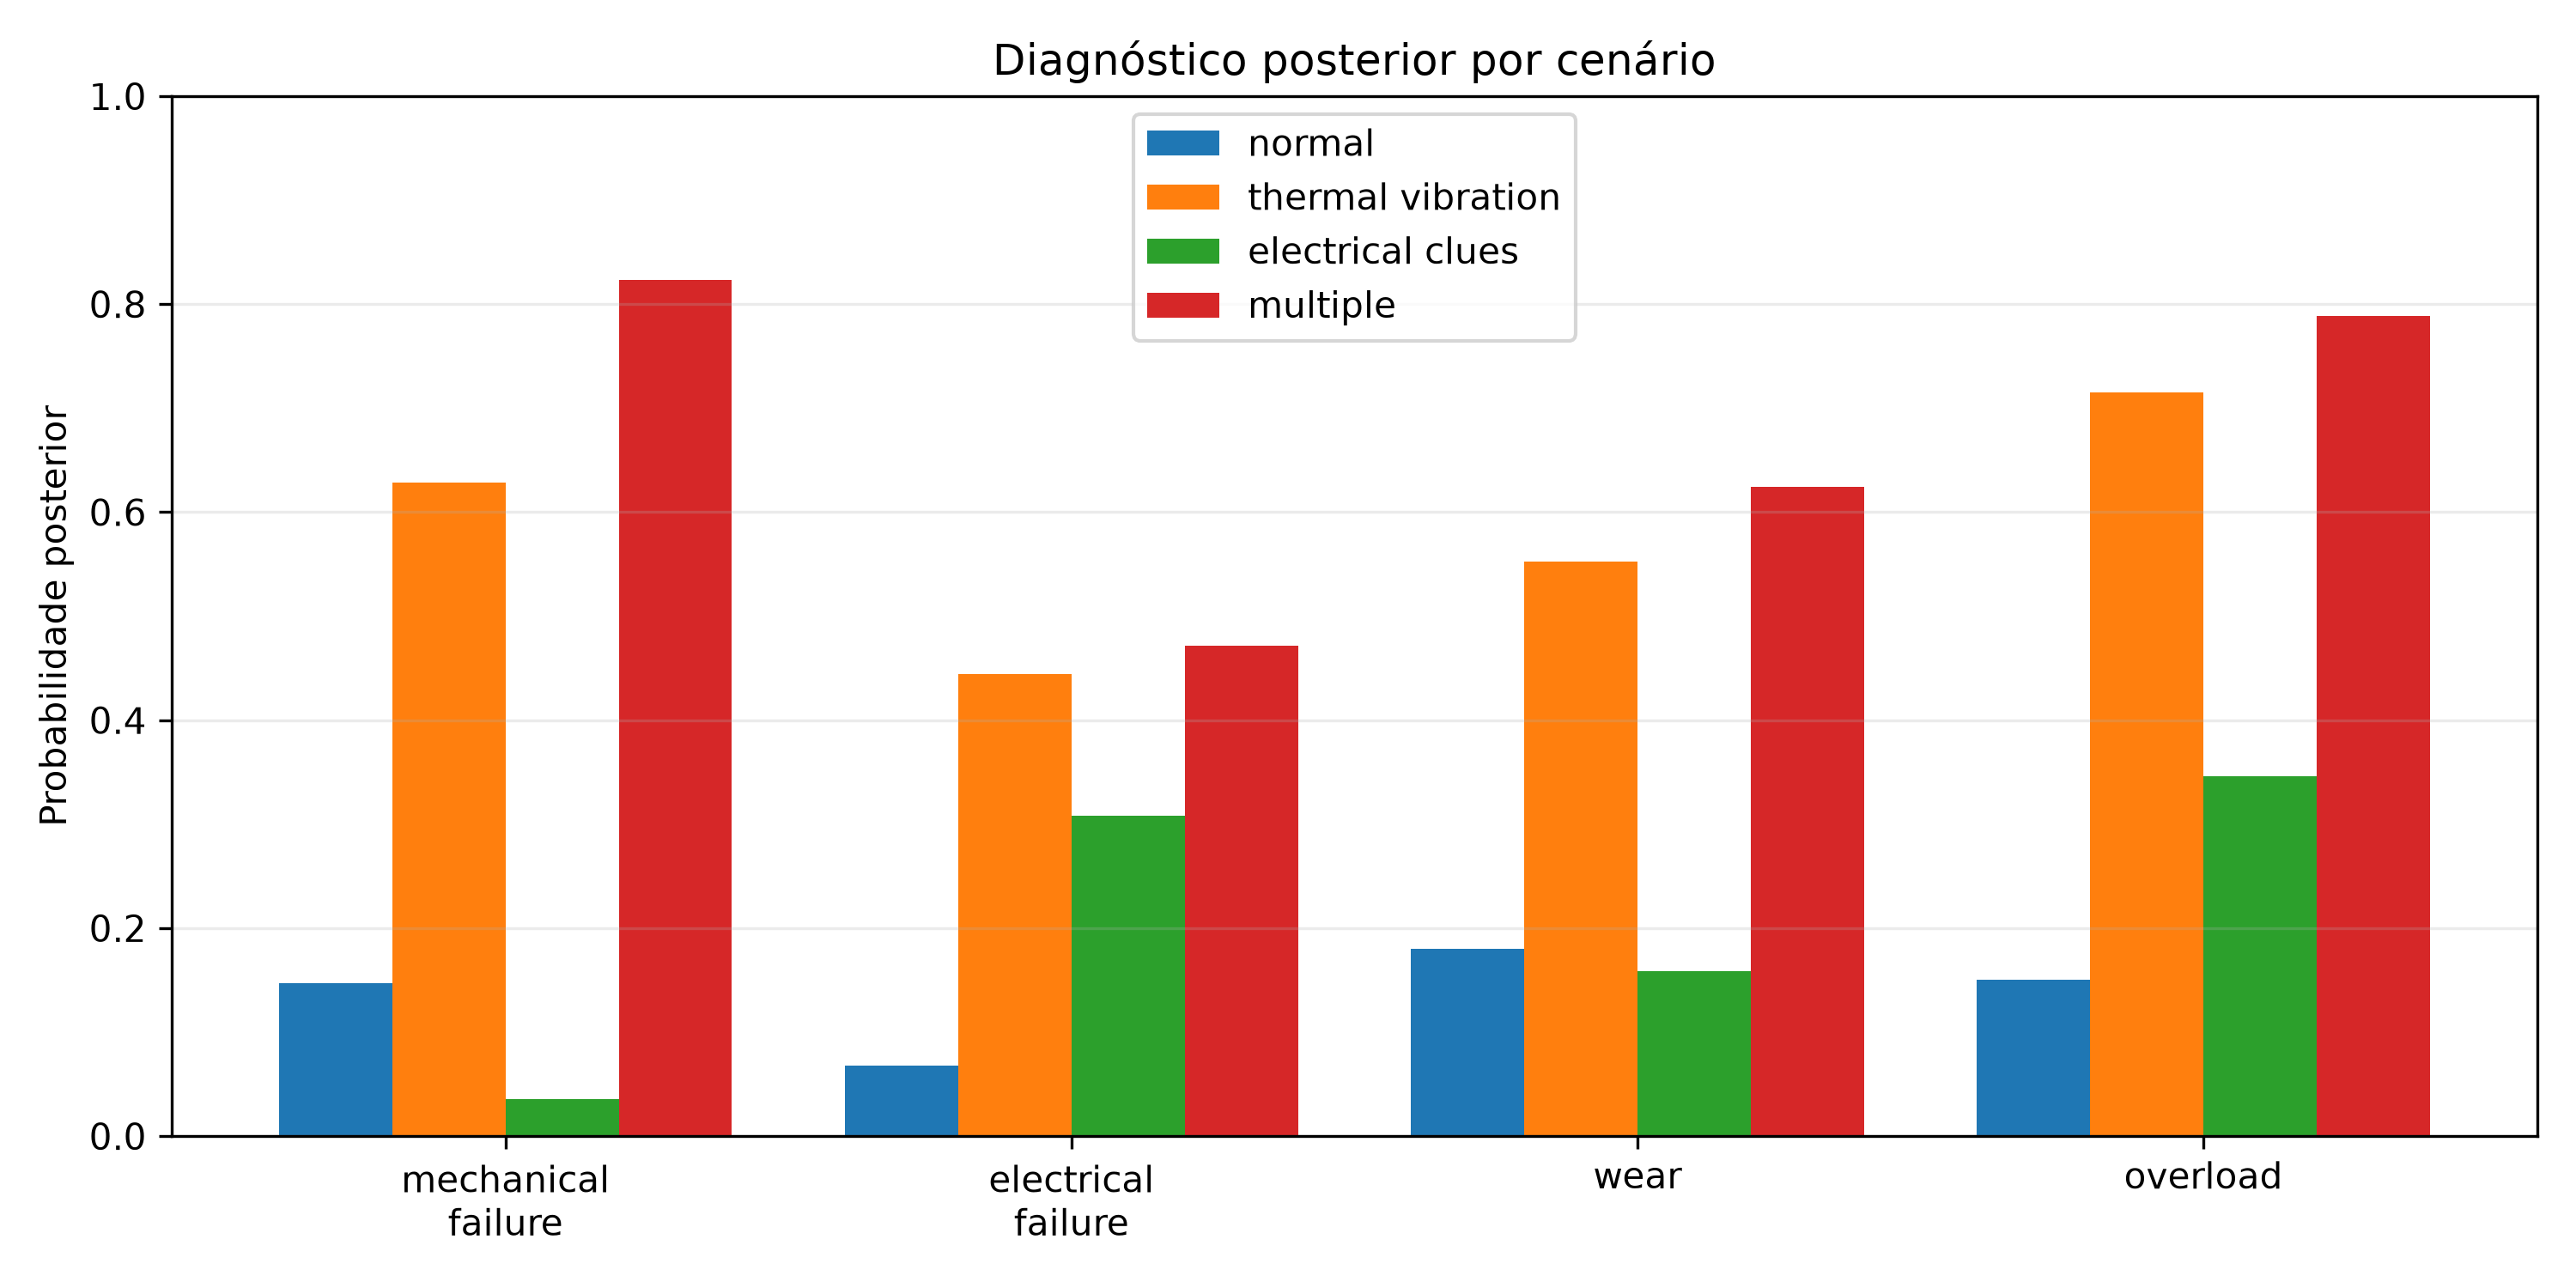
\includegraphics[width=.9\linewidth]{results/posterior_probabilities.png}\caption{Comparação dos diagnósticos posteriores.}\end{figure}
Na análise de sensibilidade, mantendo temperatura alta, acrescentar vibração alta elevou $P(\text{falha mecânica})$ em 0,5235. O resultado mostra atualização coerente: evidências correlacionadas com diferentes causas aumentam o diagnóstico, enquanto pressão normal reduz a hipótese mecânica no cenário elétrico.
\section{Considerações finais}
A rede é interpretável e permite combinar conhecimento de especialistas com sinais incompletos. A enumeração é exata, mas cresce exponencialmente com o número de variáveis; redes maiores exigem eliminação de variáveis ou amostragem. As CPTs também são uma fonte de incerteza de modelagem e deveriam ser calibradas com histórico de manutenção. Referências: Koller e Friedman (2009); Russell e Norvig (2021).
\end{document}
